%%%%%%%%%%%%%%%%%%%%%%%%%%%%%%%%%%%%%%%%%%%%%%%%%%%%%%%%%%%%%%%%%%%%%%
%%%%%%%%%%%%%%%%%%%%%%%%%%%%%%%%%%%%%%%%%%%%%%%%%%%%%%%%%%%%%%%%%%%%%%
%%%%%%%%%%%%%%%%%%%%%%%%%%%%%%%%%%%%%%%%%%%%%%%%%%%%%%%%%%%%%%%%%%%%%%
%%%%%%%%%%%%%%%%%%%%%%%%%%%%%%%%%%%%%%%%%%%%%%%%%%%%%%%%%%%%%%%%%%%%%%
\chapter{Asservissements linéaires des systèmes\label{chap-asservis}}
%%%%%%%%%%%%%%%%%%%%%%%%%%%%%%%%%%%%%%%%%%%%%%%%%%%%%%%%%%%%%%%%%%%%%%
%%%%%%%%%%%%%%%%%%%%%%%%%%%%%%%%%%%%%%%%%%%%%%%%%%%%%%%%%%%%%%%%%%%%%%
%%%%%%%%%%%%%%%%%%%%%%%%%%%%%%%%%%%%%%%%%%%%%%%%%%%%%%%%%%%%%%%%%%%%%%
%%%%%%%%%%%%%%%%%%%%%%%%%%%%%%%%%%%%%%%%%%%%%%%%%%%%%%%%%%%%%%%%%%%%%%

\minitoc
\newpage
%%%%%%%%%%%%%%%%%%%%%%%%%%%%%%%%%%%%%%%%%%%%%%%%%%%%%%%%%%%%%%%%%%%%%%
%%%%%%%%%%%%%%%%%%%%%%%%%%%%%%%%%%%%%%%%%%%%%%%%%%%%%%%%%%%%%%%%%%%%%%
%%%%%%%%%%%%%%%%%%%%%%%%%%%%%%%%%%%%%%%%%%%%%%%%%%%%%%%%%%%%%%%%%%%%%%
\section{Introduction}
%%%%%%%%%%%%%%%%%%%%%%%%%%%%%%%%%%%%%%%%%%%%%%%%%%%%%%%%%%%%%%%%%%%%%%
%%%%%%%%%%%%%%%%%%%%%%%%%%%%%%%%%%%%%%%%%%%%%%%%%%%%%%%%%%%%%%%%%%%%%%
%%%%%%%%%%%%%%%%%%%%%%%%%%%%%%%%%%%%%%%%%%%%%%%%%%%%%%%%%%%%%%%%%%%%%%

\begin{figure}[!h]
    \centering
        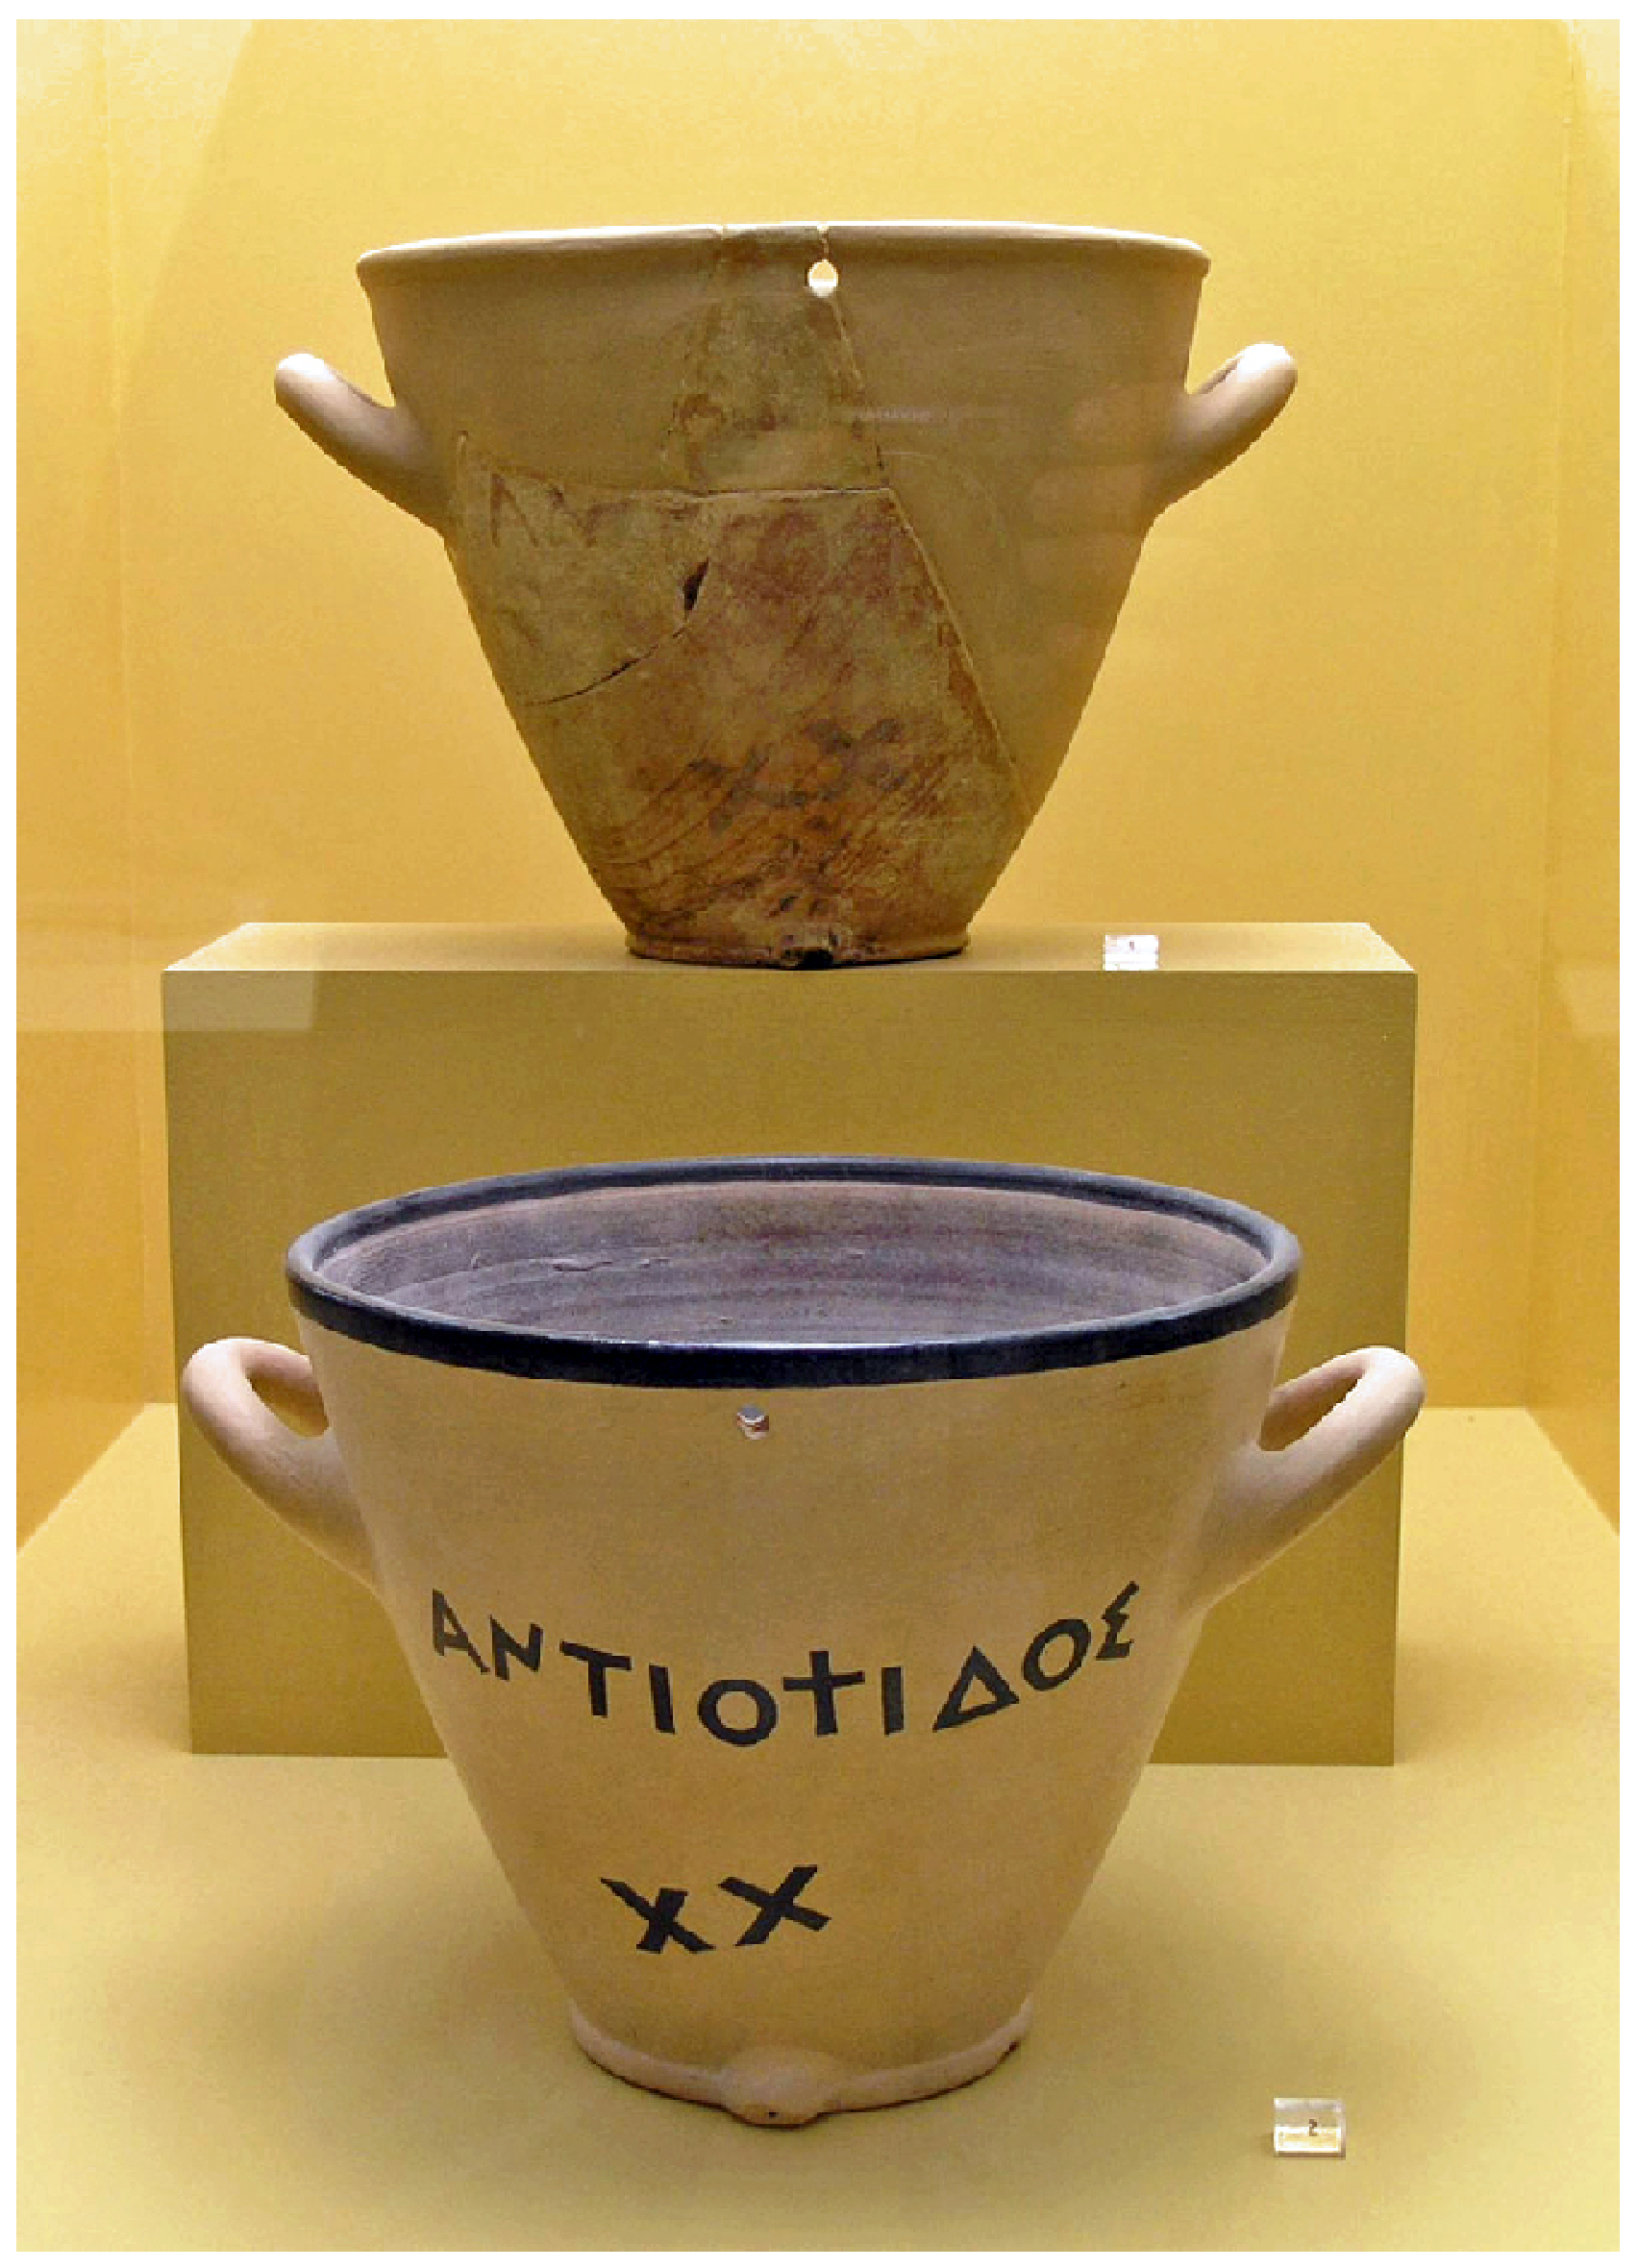
\includegraphics[width=0.45\linewidth,height=10cm]{fig/AGMA_Clepsydre_m.eps}
        \label{fig-clep}
        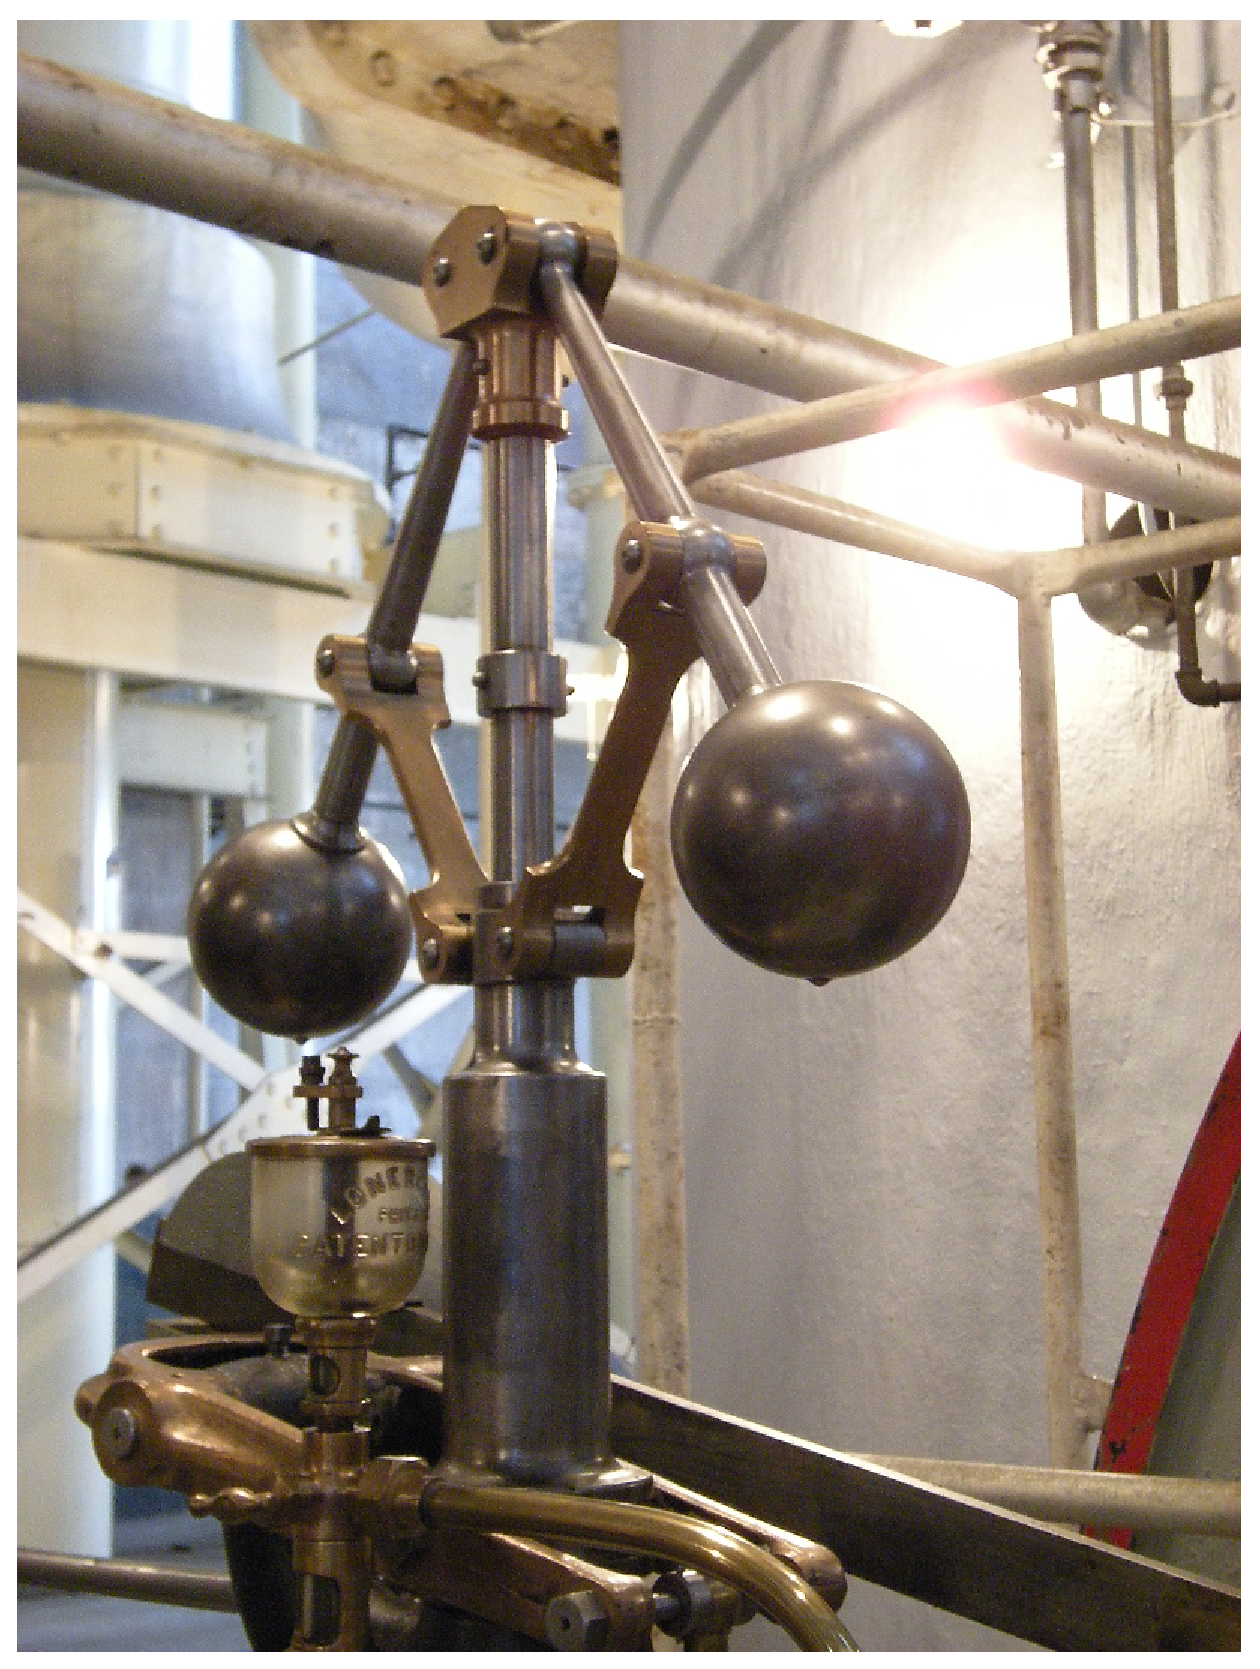
\includegraphics[width=0.45\linewidth,height=10cm]{fig/Georgetown_PowerPlant_Museum_m.eps}
        \label{fig-watt}
    \caption{Exemples historiques de régulateurs. (gauche) Clepsydre athénienne (d'après \cite{clep}) 
                                                  (droite) Régulateur de vitesse de Watt (d'après \cite{watt})\label{fig-hist}}
\end{figure}

La \textbf{régulation}\ldots
L'\textbf{asservissement}\ldots


%%%%%%%%%%%%%%%%%%%%%%%%%%%%%%%%%%%%%%%%%%%%%%%%%%%%%%%%%%%%%%%%%%%%%%
%%%%%%%%%%%%%%%%%%%%%%%%%%%%%%%%%%%%%%%%%%%%%%%%%%%%%%%%%%%%%%%%%%%%%%
%%%%%%%%%%%%%%%%%%%%%%%%%%%%%%%%%%%%%%%%%%%%%%%%%%%%%%%%%%%%%%%%%%%%%%
\section{Organisation d'un asservissement}
%%%%%%%%%%%%%%%%%%%%%%%%%%%%%%%%%%%%%%%%%%%%%%%%%%%%%%%%%%%%%%%%%%%%%%
%%%%%%%%%%%%%%%%%%%%%%%%%%%%%%%%%%%%%%%%%%%%%%%%%%%%%%%%%%%%%%%%%%%%%%
%%%%%%%%%%%%%%%%%%%%%%%%%%%%%%%%%%%%%%%%%%%%%%%%%%%%%%%%%%%%%%%%%%%%%%

\subsection{Schémas fonctionnels associés aux systèmes asservis}

\begin{figure}[!h]
%%%%%%%%%%%%%%%%%%%%%%%%%%%%%%%%%%%%%%%%%%%%%%%%%%%%%%%%%%%%%%%%%%%%%%
%   Nom des noeuds
%                                      
%   E ---- a ---- b ---- c ---- S
%          |                |
%          |                |
%            ---- d ------- 
% E : entrée
% a : comparateur
% b : correcteur
% c : système
% S : sortie
% d : capteur
% r : noeud décalé pour le retour
%%%%%%%%%%%%%%%%%%%%%%%%%%%%%%%%%%%%%%%%%%%%%%%%%%%%%%%%%%%%%%%%%%%%%%
%\begin{center}
%    \begin{tikzpicture}
%        \sbEntree{E}
%        \sbComp{a}{E}
%        \sbRelier[$E(p)$]{E}{a}           % entree
%        \sbBloc[3]{b}{$C(p)$}{a}
%        \sbRelier[$\epsilon(p)$]{a}{b}    % ecart
%        \sbBloc[3]{c}{$H(p)$}{b}
%        \sbRelier[$U(p)$]{b}{c}           % commande
%        \sbSortie[4]{S}{c}
%        \sbRelier{c}{S}
%        \sbNomLien[0.8]{S}{$S(p)$}
%        \sbDecaleNoeudy[6]{b-c}{r}
%        \sbBlocr[-1.6]{d}{$G(p)$}{r}
%        \sbRelieryx{c-S}{d}              
%        \sbRelierxy[$M(p)$]{d}{a}         % mesure (image de S)
%        \node[yshift=-0.8em] at (b.south) {\small Correcteur};
%        \node[yshift=-0.8em] at (c.south) {\small Système};
%        \node[yshift=-0.8em] at (d.south) {\small Capteur};
%        \node[yshift=-0.8em,xshift=0.5em] at (E.south) {\small Consigne};
%        \node[yshift=-0.8em] at (S.south) {\small Sortie};
%    \end{tikzpicture}
%\end{center}

%avec cadre régulateur
\begin{center}
\tikzsetnextfilename{reg_1-chap4_ext}
    \begin{tikzpicture}
        \sbEntree{E}
        \sbComp{a}{E}
        \sbRelier[$E(p)$]{E}{a}           % entree
        \sbBloc[3]{b}{$C(p)$}{a}
        \sbRelier[$\epsilon(p)$]{a}{b}    % ecart
        \sbBloc[4.2]{c}{$H(p)$}{b}
        \sbRelier[$U(p)$]{b}{c}           % commande
        \sbSortie[4]{S}{c}
        \sbRelier{c}{S}
        \sbNomLien[0.8]{S}{$S(p)$}
        \sbDecaleNoeudy[7]{b-c}{r}
        \sbBlocr[-1.6]{d}{$G(p)$}{r}
        \sbRelieryx{c-S}{d}              
        \sbRelierxy[$M(p)$]{d}{a}         % mesure (image de S)
        \node[yshift=-0.8em] at (b.south) {\small Correcteur};
        \node[yshift=-0.8em] at (c.south) {\small Système};
        \node[yshift=-0.8em] at (d.south) {\small Capteur};
        \draw[dashed,very thick,blue] (1.15,-1.8) rectangle node[blue,xshift=-1.999999999em,yshift=4em] {\textbf{Régulateur}} (4.9,1);
        \node[yshift=-0.8em,xshift=0.5em] at (E.south) {\small Consigne};
        \node[yshift=-0.8em] at (S.south) {\small Sortie};
    \end{tikzpicture}
\end{center}
\caption{\label{fig-reg}}
\end{figure}

%%%%%%%%%%%%%%%%%%%%%%%%%%%%%%%%%%%%%%%%%%%%%%%%%%%%%%%%%%%%%%%%%%%%%%
%   Nom des noeuds
%                                      
%                                      
%   E ---- a ---- b ---- c ---- d ---- e ---- S
%                 |                       |
%                 |                       |
%                  --------- f -----------
% E : entrée
% a : adaptateur 
% b : comparateur
% c : correcteur
% d : actionneur
% e : système
% S : sortie
% f : capteur
% r : noeud décalé pour le retour
%%%%%%%%%%%%%%%%%%%%%%%%%%%%%%%%%%%%%%%%%%%%%%%%%%%%%%%%%%%%%%%%%%%%%%
%\begin{center}
%    \begin{tikzpicture}
%        \sbEntree{E}
%        \sbBloc[3]{a}{$A_d(p)$}{E}
%        \sbRelier[$E(p)$]{E}{a}
%        \sbComp{b}{a}
%        \sbRelier{a}{b}
%        \sbBloc[3]{c}{$C(p)$}{b}
%        \sbRelier[$\epsilon(p)$]{b}{c}
%        \sbBloc[3]{d}{$A_c(p)$}{c}
%        \sbRelier[$\epsilon'(p)$]{c}{d}
%        \sbBloc[3]{e}{$H(p)$}{d}
%        \sbRelier[$U(p)$]{d}{e}
%        \sbSortie[4]{S}{e}
%        \sbRelier{e}{S}
%        \sbDecaleNoeudy[5]{d}{r}
%        \sbBlocr[-1.6]{f}{$G(p)$}{r}
%        \sbRelieryx{e-S}{f}              
%        \sbRelierxy[$M(p)$]{f}{b}        % Mesure
%        \sbNomLien[0.8]{S}{$S(p)$}
%        \node[yshift=-0.8em] at (a.south) {\small Adaptateur};
%        \node[yshift=-0.8em] at (c.south) {\small Correcteur};
%        \node[yshift=-0.8em] at (d.south) {\small Actionneur};
%        \node[yshift=-0.8em] at (e.south) {\small Système};
%        \node[yshift=-0.8em] at (f.south) {\small Capteur};
%        \node[yshift=-0.8em,xshift=0.5em] at (E.south) {\small Consigne};
%        \node[yshift=-0.8em] at (S.south) {\small Sortie};
%    \end{tikzpicture}
%\end{center}

%%%%%%%%%%%%%%%%%%%%%%%%%%%%%%%%%%%%%%%%%%%%%%%%%%%%%%%%%%%%%%%%%%%%%%
%   Nom des noeuds
%                                      P
%                                      |
%                                      |
%   E ---- a ---- b ---- c ---- d ---- e ---- f ---- S
%                 |                              |
%                 |                              |
%                  ------------ g ---------------
% E : entrée
% a : adaptateur 
% b : comparateur
% c : correcteur
% d : actionneur
% e : sommateur (perturbation)
% P : perturbation
% f : système 
% S : sortie
% g : capteur
% r : noeud décalé pour le retour
%%%%%%%%%%%%%%%%%%%%%%%%%%%%%%%%%%%%%%%%%%%%%%%%%%%%%%%%%%%%%%%%%%%%%%
\begin{landscape}
\vspace*{\fill}
\begin{center}
\tikzsetnextfilename{asser-chap4_ext}
    \begin{tikzpicture}
        \sbEntree{E}
        \sbBloc[3]{a}{$A_d(p)$}{E}
        \sbRelier[$E(p)$]{E}{a}
        \sbComp{b}{a}
        \sbRelier{a}{b}
        \sbBloc[3]{c}{$C(p)$}{b}
        \sbRelier[$\epsilon(p)$]{b}{c}
        \sbBloc[3]{d}{$A_c(p)$}{c}
%        \sbRelier[$\epsilon'(p)$]{c}{d}
        \sbRelier{c}{d}
        \sbSumh[6.7]{e}{d}
        \sbDecaleNoeudy[-3]{e}{P}
        \sbRenvoiF[-3]{P}{e}{$P(p)$}
        \sbRelier[$U(p)$]{d}{e}
        \sbBloc{f}{$H(p)$}{e}
        \sbRelier{e}{f}
        \sbSortie[4]{S}{f}
        \sbRelier{f}{S}
        \sbDecaleNoeudy[5]{c}{r}
        \sbBlocr[-1.6]{g}{$G(p)$}{r}
        \sbRelieryx{f-S}{g}              
        \sbRelierxy[$M(p)$]{g}{b}        
        \sbNomLien[0.8]{S}{$S(p)$}
        \node[yshift=-0.8em] at (a.south) {\small Adaptateur};
        \node[yshift=-0.8em] at (c.south) {\small Correcteur};
        \node[yshift=-0.8em] at (d.south) {\small Actionneur};
        \node[yshift=-0.8em] at (f.south) {\small Système};
        \node[yshift=-0.8em] at (g.south) {\small Capteur};
        \node[yshift=-0.8em,xshift=0.5em] at (E.south) {\small Consigne};
        \node[yshift=-0.8em] at (S.south) {\small Sortie};
        \node[yshift=2em,xshift=2.8em] at (P.east) {\small Perturbation};
        \draw[dashed,very thick,blue](-0.8,-4) 
         rectangle node[blue,xshift=-3.2em,yshift=7em]{\textbf{Chaîne d'information}}(6.9,2.5);
        \draw[dashed,very thick,red](7.3,-4)
         rectangle node[red,xshift=-5.9em,yshift=7em]  {\textbf{Chaîne d'énergie}    }(15.9,2.5);
         \draw[very thick,green!50!black,dashed,-latex] (4,1)   -- node[green!50!black,above] {Chaîne direct} (14,1) ;
         \draw[very thick,green!50!black,dashed,-latex] (14,-3.7) -- node[green!50!black,above] {Chaîne de retour} (4,-3.7) ;
    \end{tikzpicture}
\end{center}
    \captionof{figure}{Décomposition en chaîne d'information et chaîne 
                       d'énergie d'un schéma bloc d'asservissement complet\label{fig-asser}}
\vspace*{\fill}
\end{landscape}

\begin{table}[!h]
\begin{center}
    \begin{tabular}{M{3cm}M{8cm}M{4cm}N}
        \hhline{===}
        Composants      & Description & Fonction de transfert ou signal associés &\\[2em]
        \hhline{===}
        Consigne/Entrée & La valeur que l'on souhaite atteindre en sortie du système asservi.
                          Cette consigne peut être constante ou dépendante du temps. 
                        & $E(p)$                                                 &\\[5em]
        \hline
        Adaptateur      & Adapte le signal de consigne à l'image de la sortie.           
                        & $A_d(p)$                                               &\\[3em]
        \hline
        Correcteur      & \'Elabore à partir du signal d'écart $\epsilon(p)$ 
                          la commande $U(p)$ ou la grandeur réglante du système.
                        & $C(p)$                                                 & \\[3em]
        \hline
        Actionneur      & L'organe d'action qui apporte l'énergie au système.
                        & $A_c(p)$                                               &\\[3em]
        \hline
        Système         & Le système que l'on souhaite contrôler et/ou asservir
                                      & $H(p)$                                   &\\[3em]
        \hline
        Régulateur      & Le régulateur se compose d'un comparateur qui élabore le signal d'écart $\epsilon(p)$ 
                          à partir de la consigne et de la mesure, formellement le régulateur incorpore le correcteur 
                          et du correcteur.
                                      & $\epsilon(p)$                            &\\[3em]
        \hline
        Perturbation    & Phénomène physique intervenant sur le système qui en modifie la sortie
                                      & $P(p)$                                   &\\[3em]
        \hline
        Capteur         &  Le capteur prélève le sortie pour en donner une image (la mesure) 
                           utile au régulateur. Intervenant dans la boucle ouverte, son étude 
                           est indispensable pour la caractérisation des performances du système asservi.
                                      & $G(p)$                                   &\\[3em]
        \hline
        Mesure          & Le signal de la mesure de la sortie ou image de la sortie
                          élaboré par le capteur.
                                      & $M(p)$                                   &\\[3em]  
        \hline
        Sortie          & Le signal de sortie du système que l'on souhaite régulé et/ou asservir
                                      & $S(p)$                                   &\\[3em]
        \hhline{===}
    \end{tabular}
\end{center}
\caption{Terminologie et définition associés à l'asservissement des systèmes.\label{tab-asser}}
\end{table}

\clearpage

\subsection{Fonctions de transferts associées à un système asservi}

%Chacuns des blocs du schéma fonctionnel d'un asservissement~\cref{fig-asser} permet 
%de définir une fonction de transfert reliant localement une entrée et une sortie.
%Nous allons définir quelques fonctions de transferts fondamentales à 
%l'étude d'un système asservi :

\paragraph{Fonction de transfert de la chaîne directe}

La~\gls{ftcd}, que nous noterons $H_{CD}(p)$ est liée à 
la chaîne d'action de l'asservissement. Elle lie la sortie $S(p)$ à l'écart $\epsilon(p)$.
Formellement,
\begin{bequation}[ams align]
H_{CD}(p)=\dfrac{S(p)}{\epsilon(p)}
\end{bequation}

\paragraph{Fonction de transfert de la chaîne de retour}

La~\gls{ftcr}, que nous noterons $H_{CR}(p)$ est 
liée à la chaîne de mesure de l'asservissement. Elle lie l'image de la sortie $M(p)$ à la sortie $S(p)$ 
Formellement,
\begin{bequation}[ams align]
H_{CR}(p)=\dfrac{M(p)}{S(p)}
\end{bequation}
Dans le cas d'un retour unitaire $H_{CR}(p)=1$, c'est à dire que la sortie est la consigne sont de même 
nature.

\paragraph{Fonction de transfert en boucle ouverte}

La~\gls{ftbo}, que nous noterons $H_{BO}(p)$ correspond
à la fonction de transfert du système non asservi. Elle lie l'image de la sortie $M(p)$ à l'écart $\epsilon(p)$.
Formellement,
\begin{bequation}[ams align]
H_{BO}(p)=\dfrac{M(p)}{\epsilon(p)}=\dfrac{M(p)}{S(p)}\dfrac{S(p)}{\epsilon(p)}=H_{CR}(p)H_{CD}(p)
\end{bequation}
Dans le cas d'un retour unitaire on obtient $H_{BO}(p)=H_{CD}(p)$

\paragraph{Fonction de transfert en boucle fermée}

La~\gls{ftbf}, que nous noterons $H_{BF}(p)$ correspond
explicitement à la fonction de transfert du système asservi. Elle lie la sortie du système $S(p)$ 
à la consigne $E(p)$. Formellement et en appliquant la réduction des schémas blocs (c.f~\cref{sec-boucle}),
\begin{bequation}[ams align]
    H_{BF}(p)=\dfrac{S(p)}{E(p)}=\dfrac{H_{CD}(p)}{1+H_{CR}(p)H_{CD}(p)}=\dfrac{H_{CD}(p)}{1+H_{BO}(p)}
\end{bequation}

Remarquons que dans le cas d'une boucle de contre réaction unitaire (c.a.d $H_{CR}(p)=1$),
la~\gls{ftbf} se réduit à :
$$
H_{BF}(p)=\dfrac{H_{BO}(p)}{1+H_{BO}(p)}
$$

%%%%%%%%%%%%%%%%%%%%%%%%%%%%%%%%%%%%%%%%%%%%%%%%%%%%%%%%%%%%%%%%%%%%%%
%%%%%%%%%%%%%%%%%%%%%%%%%%%%%%%%%%%%%%%%%%%%%%%%%%%%%%%%%%%%%%%%%%%%%%
%%%%%%%%%%%%%%%%%%%%%%%%%%%%%%%%%%%%%%%%%%%%%%%%%%%%%%%%%%%%%%%%%%%%%%
\section{Asservissement des SLCI modèles}
%%%%%%%%%%%%%%%%%%%%%%%%%%%%%%%%%%%%%%%%%%%%%%%%%%%%%%%%%%%%%%%%%%%%%%
%%%%%%%%%%%%%%%%%%%%%%%%%%%%%%%%%%%%%%%%%%%%%%%%%%%%%%%%%%%%%%%%%%%%%%
%%%%%%%%%%%%%%%%%%%%%%%%%%%%%%%%%%%%%%%%%%%%%%%%%%%%%%%%%%%%%%%%%%%%%%

%%%%%%%%%%%%%%%%%%%%%%%%%%%%%%%%%%%%%%%%%%%%%%%%%%%%%%%%%%%%%%%%%%%%%%
%%%%%%%%%%%%%%%%%%%%%%%%%%%%%%%%%%%%%%%%%%%%%%%%%%%%%%%%%%%%%%%%%%%%%%
\subsection{Asservissement d'un intégrateur}
%%%%%%%%%%%%%%%%%%%%%%%%%%%%%%%%%%%%%%%%%%%%%%%%%%%%%%%%%%%%%%%%%%%%%%
%%%%%%%%%%%%%%%%%%%%%%%%%%%%%%%%%%%%%%%%%%%%%%%%%%%%%%%%%%%%%%%%%%%%%%

Considérons un système intégrateur asservi et régi par le schéma-bloc suivant :
\begin{center}
\tikzsetnextfilename{asser_int-chap4_ext}
    \begin{tikzpicture}
        \sbEntree{E}
        \sbComp{a}{E}
        \sbRelier[$E(p)$]{E}{a}
       % \sbBloc{b}{$C(p)$}{a}
        \sbBloc{b}{$\dfrac{K}{p}$}{a}
        \sbRelier{a}{b}
        \sbSortie[4]{S}{b}
        \sbRelier{b}{S}
        \sbRenvoi{b-S}{a}{}
        \sbNomLien[0.8]{S}{$S(p)$}
    \end{tikzpicture}
\end{center}

La fonction de transfert en boucle ouverte $H(p)$ est telle que :
$$
H(p)=\dfrac{K}{p}
$$
avec $K$ le gain statique. 
Les~\gls{ftbo} et~\gls{ftbf} sont respectivement :
$$
H_{BO}(p)=H(p)
$$
et
$$
H_{BF}(p)=\dfrac{H(p)}{1+H(p)}=\dfrac{K}{p+K}
$$

L'étude de la réponse temporelle d'un intégrateur nous a permis de conclure sur 
son instabilité intrisèque.

%%%%%%%%%%%%%%%%%%%%%%%%%%%%%%%%%%%%%%%%%%%%%%%%%%%%%%%%%%%%%%%%%%%%%%
%%%%%%%%%%%%%%%%%%%%%%%%%%%%%%%%%%%%%%%%%%%%%%%%%%%%%%%%%%%%%%%%%%%%%%
\subsection{Asservissement d'un système du premier ordre}
%%%%%%%%%%%%%%%%%%%%%%%%%%%%%%%%%%%%%%%%%%%%%%%%%%%%%%%%%%%%%%%%%%%%%%
%%%%%%%%%%%%%%%%%%%%%%%%%%%%%%%%%%%%%%%%%%%%%%%%%%%%%%%%%%%%%%%%%%%%%%

Considérons un système du premier ordre asservi et régi par le schéma-bloc suivant :
\begin{center}
\tikzsetnextfilename{asser_1er-chap4_ext}
    \begin{tikzpicture}
        \sbEntree{E}
        \sbComp{a}{E}
        \sbRelier[$E(p)$]{E}{a}
       % \sbBloc{b}{$C(p)$}{a}
        \sbBloc{b}{$\dfrac{K}{1+\tau p}$}{a}
        \sbRelier{a}{b}
        \sbSortie[4]{S}{b}
        \sbRelier{b}{S}
        \sbRenvoi{b-S}{a}{}
        \sbNomLien[0.8]{S}{$S(p)$}
    \end{tikzpicture}
\end{center}
La fonction de transfert en boucle ouverte $H(p)$ du procédé est alors tel que:
$$
H(p)=\dfrac{K}{1+\tau p}
$$
où $K$ est le gain statique et $\tau$ la constante de temps du système en boucle ouverte.
On a alors pour~\gls{ftbo} et~\gls{ftbf} respectivement :
$$
H_{BO}(p)=H(p)
$$
et 
$$
H_{BF}(p)=\dfrac{H(p)}{1+H(p)}=\dfrac{K}{(1+K)+\tau p}
$$
Remarquons que la~\gls{ftbf} reste du premier ordre. Sous une forme canonique
cette fonction de transfert devient :
$$
H_{BF}(p)=\dfrac{\dfrac{K}{1+K}}{1+\dfrac{\tau}{1+K}p}=\dfrac{K_{BF}}{1+\tau_{BF} p}
$$
où $K_{BF}$ est le gain statique et $\tau_{BF}$ la constante de temps sont les 
paramètres du système en boucle fermée.
Par identification, on alors les rélations suivantes entre les paramètres du premier ordre 
de la~\gls{ftbo} et les paramètres du premier ordre de la~\gls{ftbf} :
\begin{align*}
       K_{BF}&=\dfrac{K}{1+K}\\
    \tau_{BF}&=\dfrac{\tau}{1+K}
\end{align*}

Constatons que le gain statique en boucle ouverte $K$ intervient 
dans la définition du gain statique $K_{BF}$ et de la constante de temps $\tau_{BF}$ en boucle fermée. 
Ainsi en modifiant le paramètre $K$, il est possible de jouer sur les deux paramètres régissant la boucle fermée.
Pour $K>0$, le domaine de définition des paramètres du système en boucle fermée sont  $K_{BF}\in[0,1[$ et  $\tau_{BF}\in]0,\tau]$

%%%%%%%%%%%%%%%%%%%%%%%%%%%%%%%%%%%%%%%%%%%%%%%%%%%%%%%%%%%%%%%%%%%%%%
%%%%%%%%%%%%%%%%%%%%%%%%%%%%%%%%%%%%%%%%%%%%%%%%%%%%%%%%%%%%%%%%%%%%%%
\subsection{Asservissement d'un système du second ordre}
%%%%%%%%%%%%%%%%%%%%%%%%%%%%%%%%%%%%%%%%%%%%%%%%%%%%%%%%%%%%%%%%%%%%%%
%%%%%%%%%%%%%%%%%%%%%%%%%%%%%%%%%%%%%%%%%%%%%%%%%%%%%%%%%%%%%%%%%%%%%%

Considérons un système du second ordre asservi et régi par le schéma-bloc suivant :
\begin{center}
\tikzsetnextfilename{asser_2nd-chap4_ext}
    \begin{tikzpicture}
        \sbEntree{E}
        \sbComp{a}{E}
        \sbRelier[$E(p)$]{E}{a}
       % \sbBloc{b}{$C(p)$}{a}
        \sbBloc{b}{$H(p)=\dfrac{K\omega^2_0}{\omega^2_0+2\xi\omega_0p+p^2}$}{a}
        \sbRelier{a}{b}
        \sbSortie[4]{S}{b}
        \sbRelier{b}{S}
        \sbRenvoi{b-S}{a}{}
        \sbNomLien[0.8]{S}{$S(p)$}
    \end{tikzpicture}
\end{center}
La fonction de transfert en boucle ouverte du procédé $H(p)$ est tel que:
$$
H(p)=\dfrac{K\omega^2_0}{\omega^2_0+2\xi\omega_0p+p^2}
$$
où $K$ est le gain statique, $\omega_0$ la pulsation propre et $\xi$ 
le coefficient d'amortissement du système en boucle ouverte.
Les~\gls{ftbo} et~\gls{ftbf} sont respectivement :
$$
H_{BO}(p)=H(p)
$$
et 
$$
H_{BF}(p)=\dfrac{H(p)}{1+H(p)}=\dfrac{K\omega^2_0}{\omega^2_0(1+K)+2\xi\omega_0p+p^2}
$$
Une nouvelle fois, nous constatons que la fonction de transfert en boucle fermée est du même ordre
que celle en boucle ouverte. Sous une forme canonique la~\gls{ftbf} devient :
$$
H_{BF}(p)=\dfrac{K\omega^2_0}{\omega^2_0(1+K)+2\xi\omega_0p+p^2}=
\dfrac{K_{BF}\omega^2_{0,BF}}{\omega^2_{0,BF}(1+K_{BF})+2\xi_{BF}\omega_{0,BF}p+p^2}
$$
Par identification, on alors les rélations suivantes entre les paramètres du premier ordre 
de la~\gls{ftbo} et les paramètres du premier ordre de la~\gls{ftbf} :
\begin{align*}
       K_{BF}&=\dfrac{K}{1+K}\\
    \omega_{0,BF}&=\omega_0\sqrt{1+K}\\
    \xi_{BF}&=\dfrac{\xi}{\sqrt{1+K}}
\end{align*}

%%%%%%%%%%%%%%%%%%%%%%%%%%%%%%%%%%%%%%%%%%%%%%%%%%%%%%%%%%%%%%%%%%%%%%
%%%%%%%%%%%%%%%%%%%%%%%%%%%%%%%%%%%%%%%%%%%%%%%%%%%%%%%%%%%%%%%%%%%%%%
%%%%%%%%%%%%%%%%%%%%%%%%%%%%%%%%%%%%%%%%%%%%%%%%%%%%%%%%%%%%%%%%%%%%%%
\section{Performances des systèmes en boucle ouverte}
%%%%%%%%%%%%%%%%%%%%%%%%%%%%%%%%%%%%%%%%%%%%%%%%%%%%%%%%%%%%%%%%%%%%%%
%%%%%%%%%%%%%%%%%%%%%%%%%%%%%%%%%%%%%%%%%%%%%%%%%%%%%%%%%%%%%%%%%%%%%%
%%%%%%%%%%%%%%%%%%%%%%%%%%%%%%%%%%%%%%%%%%%%%%%%%%%%%%%%%%%%%%%%%%%%%%

\subsection{Stabilité en boucle ouverte}

\subsection{Précision en boucle ouverte}

\subsection{Rapidité en boucle ouverte}

\subsection{Dépassement en boucle }



\newpage
%%%%%%%%%%%%%%%%%%%%%%%%%%%%%%%%%%%%%%%%%%%%%%%%%%%%%%%%%%%%%%%%%%%%%%
%%%%%%%%%%%%%%%%%%%%%%%%%%%%%%%%%%%%%%%%%%%%%%%%%%%%%%%%%%%%%%%%%%%%%%
%%%%%%%%%%%%%%%%%%%%%%%%%%%%%%%%%%%%%%%%%%%%%%%%%%%%%%%%%%%%%%%%%%%%%%
\section*{Exercices du chapitre}
%%%%%%%%%%%%%%%%%%%%%%%%%%%%%%%%%%%%%%%%%%%%%%%%%%%%%%%%%%%%%%%%%%%%%%
%%%%%%%%%%%%%%%%%%%%%%%%%%%%%%%%%%%%%%%%%%%%%%%%%%%%%%%%%%%%%%%%%%%%%%
%%%%%%%%%%%%%%%%%%%%%%%%%%%%%%%%%%%%%%%%%%%%%%%%%%%%%%%%%%%%%%%%%%%%%%


\exercice{}
\question

\newpage
%%%%%%%%%%%%%%%%%%%%%%%%%%%%%%%%%%%%%%%%%%%%%%%%%%%%%%%%%%%%%%%%%%%%%%
%%%%%%%%%%%%%%%%%%%%%%%%%%%%%%%%%%%%%%%%%%%%%%%%%%%%%%%%%%%%%%%%%%%%%%
%%%%%%%%%%%%%%%%%%%%%%%%%%%%%%%%%%%%%%%%%%%%%%%%%%%%%%%%%%%%%%%%%%%%%%
\section*{Corrigé des exercices}
%%%%%%%%%%%%%%%%%%%%%%%%%%%%%%%%%%%%%%%%%%%%%%%%%%%%%%%%%%%%%%%%%%%%%%
%%%%%%%%%%%%%%%%%%%%%%%%%%%%%%%%%%%%%%%%%%%%%%%%%%%%%%%%%%%%%%%%%%%%%%
%%%%%%%%%%%%%%%%%%%%%%%%%%%%%%%%%%%%%%%%%%%%%%%%%%%%%%%%%%%%%%%%%%%%%%


